\documentclass[a0paper,portrait]{baposter}

\setlength{\paperwidth}{847mm}
\setlength{\paperheight}{1195mm}
\special{papersize=\the\paperwidth,\the\paperheight} % works in pdf/Xe/Lua
\typeout{PDF PAGE SIZE: \the\paperwidth\space x \the\paperheight}


\usepackage{lipsum}          % This is just for some blindtext
\usepackage{relsize}	       % For \smaller
\usepackage{url}			       % For \url
\usepackage{epstopdf}	       % Included EPS files automatically converted to PDF to include with pdflatex
\usepackage{multicol}        % Multi Columns
\usepackage{dcolumn}
\usepackage[table]{xcolor}
\usepackage{amsmath,amssymb} % math
\usepackage{anyfontsize}
\usepackage{caption}
\captionsetup[table]{position=top}  
\usepackage{url,graphicx,indentfirst}
\usepackage{hhline}
\usepackage{tikz}
\usepackage{adjustbox}
\usepackage{textcomp}
\usepackage{verbatim}
\usepackage{color, colortbl}
\usepackage{booktabs,siunitx}
\usepackage{csvsimple}
\usepackage{enumitem}
\usepackage[ruled,vlined]{algorithm2e}
\renewcommand{\labelitemi}{$\textcolor{aaublue1}{\LARGE\bullet}$}
\newcommand\blfootnote[1]{%
  \begingroup
  \renewcommand\thefootnote{}\footnote{#1}%
  \addtocounter{footnote}{-1}%
  \endgroup
}
%%%%


\usepackage{mathtools}



%%%%%%%%%%%%%%%%%%%%%%%%%%%%%%%%%%%%%%%%%%%%%%%%%%%%%%%%%%%%%%%%%%%%%%%%%%%%%%%%
%%% Utility functions %%%%%%%%%%%%%%%%%%%%%%%%%%%%%%%%%%%%%%%%%%%%%%%%%%%%%%%%%%
%%%%%%%%%%%%%%%%%%%%%%%%%%%%%%%%%%%%%%%%%%%%%%%%%%%%%%%%%%%%%%%%%%%%%%%%%%%%%%%%

%%% Save space in lists. Use this after the opening of the list %%%%%%%%%%%%%%%%
\renewcommand{\vec}[1]{\bm{#1}}
\newcommand{\vnabla}{\vec{\nabla}}

\renewcommand{\d}[1]{\text{d} #1}
\newcommand{\dxx}{\,\text{d}\vec{x}}
\newcommand{\dx}{\,\text{d}x}

\newcommand{\diff}[2]{\frac{\text{d}#1}{\text{d}#2}}
\newcommand{\idiff}[2]{\text{d}#1 / \text{d}#2}
\newcommand{\pdiff}[2]{\frac{\partial #1}{\partial #2}}
\newcommand{\pdifff}[2]{\frac{\partial^2 #1}{\partial #2^2}}
\newcommand{\ipdiff}[2]{\partial #1 / \partial #2}
\newcommand{\vdiff}[2]{\frac{\delta #1}{\delta #2}}
\newcommand{\ivdiff}[2]{\delta #1 / \delta #2}

%%%%%%%%%%%%%%%%%%%%%%%%%%%%%%%%%%%%%%%%%%%%%%%%%%%%%%%%%%%%%%%%%%%%%%%%%%%%%%%
%%% Document Start %%%%%%%%%%%%%%%%%%%%%%%%%%%%%%%%%%%%%%%%%%%%%%%%%%%%%%%%%%%%
%%%%%%%%%%%%%%%%%%%%%%%%%%%%%%%%%%%%%%%%%%%%%%%%%%%%%%%%%%%%%%%%%%%%%%%%%%%%%%%

\begin{document}
\typeout{Poster rendering started}

%%% General Poster Settings %%%%%%%%%%%%%%%%%%%%%%%%%%%%%%%%%%%%%%%%%%%%%%%%%%%
%%%%%% Eye Catcher, Title, Authors and University Images %%%%%%%%%%%%%%%%%%%%%%
\begin{poster}{
  columns=2,
	grid=false,
	borderColor=aaublue1,
	headerColorOne=aaublue1,
	headerColorTwo=aaublue1,
	headerFontColor=white,
  headerheight=13em,
	boxColorOne=white,
  boxpadding=1em,
	headershape=rounded,
	headerfont=\Large\textsf,
	textborder=rounded,
	background=shadetb,
  bgColorOne=aaublue2!20,
  bgColorTwo=aaublue2!80,
	headerborder=open,
  boxshade=plain,
  eyecatcher=false
}
%%% Eye Cacther %%%%%%%%%%%%%%%%%%%%%%%%%%%%%%%%%%%%%%%%%%%%%%%%%%%%%%%%%%%%%%%
{
}
%%% Title %%%%%%%%%%%%%%%%%%%%%%%%%%%%%%%%%%%%%%%%%%%%%%%%%%%%%%%%%%%%%%%%%%%%%
%{Towards Checking Dynamic Controllability \\ of Processes with Temporal Loops}
{\vspace*{1em}%
 \fontsize{26}{33}\selectfont
 \textcolor{black}{Reproducibility of LLM-based Recommender Systems Research: Worrying Observations from an Initial Analysis}}
%%% Authors %%%%%%%%%%%%%%%%%%%%%%%%%%%%%%%%%%%%%%%%%%%%%%%%%%%%%%%%%%%%%%%%%%%
{
  \vspace{1em}\textcolor{black}{\textbf{Faisal Shehzad, and Dietmar Jannach}\\
	{\smaller {University of Klagenfurt, Austria}}\\
	{\smaller {faisal.shehzad}@aau.at}, 
	{\smaller {dietmar.jannach}@aau.at}
}}
%%% Logo %%%%%%%%%%%%%%%%%%%%%%%%%%%%%%%%%%%%%%%%%%%%%%%%%%%%%%%%%%%%%%%%%%%%%%


%%%%%%%%%%%%%%%%%%%%%%%%%%%%%%%%%%%%%%%%%%%%%%%%%%%%%%%%%%%%%%%%%%
\headerbox{Motivation}{name=b1,column=0,row=0,span=1}{
 \begin{itemize}
     \item Large language models (LLMs) are shaping recommender systems research and becoming central to modern recommendation architectures.
     \item Their stochasticity and complexity introduce new reproducibility challenges.
     %\item Previous studies show that the reported details in research articles are often insufficient for reproducing results.
     \item \textbf{Goal:} Identify key reproducibility variables for LLM-based recommender systems and assess their documentation in high-ranked venues.
 \end{itemize}
}

 %%%%%%%%%%%%%%%%%%%%%%%%%%%%%%%%%%%%%%%%%%%%%%%%%%%%%%%%%%%%%%%%%%
\headerbox{Research Methodology}{name=b2,column=0,row=0,span=1, below = b1}{

\textbf{Paper Selection Process:}
\begin{itemize}
    \item Scanned 2023–2025 proceedings of high-ranked conferences and selected papers mentioning “LLM” with “recommender” or “recommendation” in the title, abstract, or introduction.
    \item Excluded papers for which all authors were affiliated with industry, as code sharing is often restricted in such cases.
    \item This criterion leads us to the selection of 64 papers.
\end{itemize}

\vspace{0.3em}

\begin{center}
\textbf{Table 1: Papers by venue}

\vspace{0.2em}

\begin{tabular}{lccccc}
\hline
Venue & RecSys & SIGIR & WWW & WSDM & KDD \\
\hline
No. of papers & 25 & 17 & 8 & 7 & 7 \\
\hline
\end{tabular}
\end{center}
}

\headerbox{Reproducibility Variables}{name=b3, column=0, span=1,below=b2}{
We use variables from prior studies and policies as reproducibility indicators. \\ [0.25cm]
With slight customization, we grouped them into two main variables.
 \begin{itemize}
    \item \textbf{General
reproducibility variables} (source code, hyperparameter ranges, train-test splits, etc.)
     \item \textbf{LLM-specific reproducibility variables} (model version, fine-tuning materials, Fine-tuning strategy, Checkpoints, Prompt type, Prompt documentation, Temperature, etc.) 
 \end{itemize}
}

%%%%%%%%%%
\headerbox{Results (1/2): General reproducibility variables}
{name=b4,span=1,below=b3,column=0}{
\begin{center}
\textbf{\large Source code}\\[-0.3em]
\end{center}


\begin{center}
    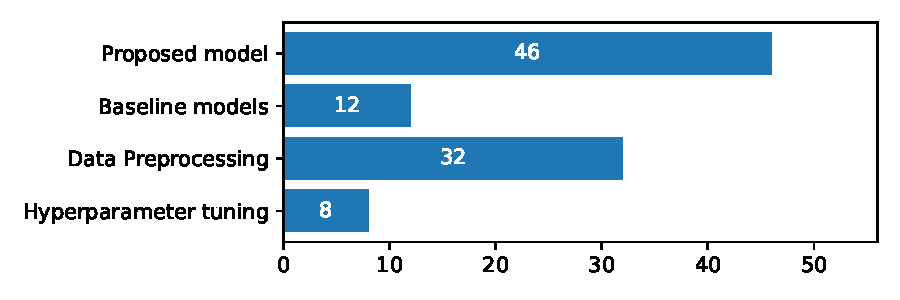
\includegraphics[width=0.7\linewidth,height=3cm]{code.pdf}
    \captionof{figure}{Code sharing statistics}
    \label{fig:code}
\end{center}

\vspace{0.1em}
\textbf{Additional observations:}
\begin{itemize}
    \item \textbf{Of 64 papers}, \textbf{49} provided code repository links; however, \textbf{3} were inaccessible, leaving \textbf{46 papers (71\%)} with available code.
    \item All repositories share proposed-model code; only \textbf{12} include baselines.
    \item Hyperparameter tuning was required for \textbf{59 papers}, but only \textbf{5} shared complete tuning scripts; \textbf{3} shared partial scripts, and \textbf{11} used fixed hyperparameters without any justification.    
    \item \textbf{For the remaining reproducibility variables}, such as hyperparameter ranges, train-test splits, and evaluation details, our findings align with previous studies; therefore, they are not reported in the poster.
\end{itemize}
}



\headerbox{Results (2/2): LLM-specific reproducibility variables }{name=b6 ,span=1,column=1}{

{ \centering
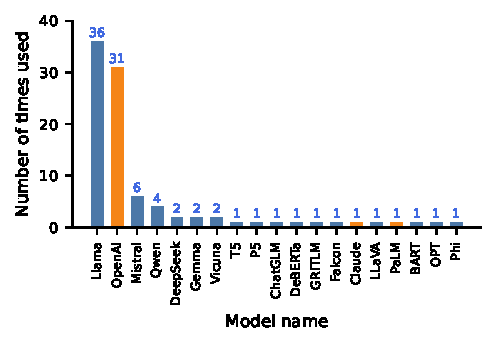
\includegraphics[width=0.75\linewidth]{llm_usuage_names.pdf}
\captionof{figure}{Frequency of model usage for closed- and open-source LLMs.}
\label{fig:llm_usage_names}
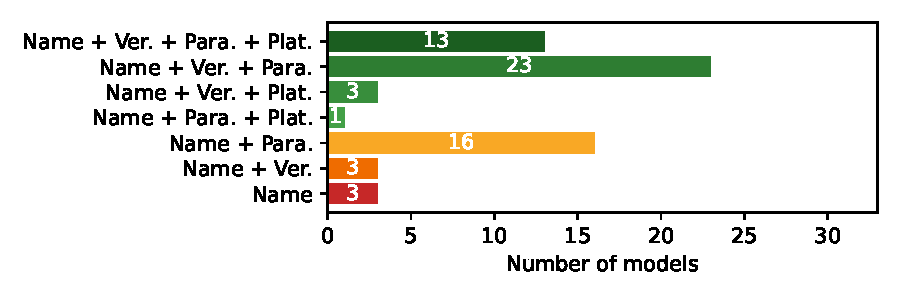
\includegraphics[width=0.75\linewidth]{open_source_llms.pdf}
  \captionof{figure}{Documentation of Open-Source Model Usages.}
  \label{fig:open_source_llms}
}
\textbf{LLM Models and Versions:}  
  \begin{itemize}
      \item Most studies \textbf{(38 papers)} use open-source models; \textbf{13} use closed-source models, \textbf{12} use both, and \textbf{1} does not report the model name.  
      \item OpenAI models are used \textbf{31 times across 24 papers}, but only \textbf{5 papers} report both version and snapshot; \textbf{24} report only the version, and \textbf{1} reports only the model name.
      \item Open-source models are used \textbf{62 times in 52 papers}, with \textbf{Llama} dominating; Figure \ref{fig:open_source_llms} summarizes how well key details are reported.
      
  \end{itemize}
\textbf{Fine-Tuning Aspects:}
    \begin{itemize}
        \item Fine-tuning is used in \textbf{39 papers}, but only \textbf{6 (15\%)} provide complete tuning materials; the rest provide partial or no materials.
        \item Checkpoints and model weights support reproduction, but only \textbf{1 paper} shares checkpoints and \textbf{3} share model weights.
        \item Tokenizer details are rarely reported: only \textbf{6 papers} provide both tokenizer name and version.
    \end{itemize}
\textbf{Prompt-Related Aspects:}
    \begin{itemize}
        \item Prompts are used in \textbf{50 papers}; \textbf{47} document them, \textbf{1} partially, and \textbf{2} provide none.
        \item Prompt templates are shared in \textbf{44 papers}; among \textbf{34 papers} with source code, \textbf{more than half (23)} include the exact template in the code.
        \item Only \textbf{5} papers report the context window length for prompt templates.
    \end{itemize}
\textbf{Temperature} affects LLM output randomness and reproducibility; \textbf{only 43.75\% of papers} report its value.    
}


%%%%%%%%%%%%%%%%%%%%%%%%%%%%%%%%%%%%%%%%%%%%%%%%%%%%%%%%%%%%%%%%%%%%%%%%
\headerbox{Conclusion \& Discussion}{name = b8, below=b6, span = 1, column=1}{

 \begin{itemize}
    \item Our findings align with prior evidence: current experimental reporting does not fully support reproducibility.
    \item Long-standing reproducibility issues persist in LLM-based studies and are further compounded by LLM-specific documentation needs.
    \item Stricter and more rigorous practices are needed to improve reproducibility.
 \end{itemize}
}

\end{poster}
\end{document}
